\section{Brugsscenarier}
\label{ParametreBrugsscenarier}
%
For at få de rejsende til at sætte deres egne ord på oplevelsen af interaktionen med en social robot defineres der tre brugsscenarier, som anses for at forekomme naturligt i en lufthavn. De tre brugsscenarier henvender sig til at den rejsende skal finde gate information, finde toiletfaciliteter og finde indkøbsmuligheder. De tre brugsscenarier gengives i \textit{wireframe} designet i \textit{Marvel}, som præsenteres på \textit{Double}s skærm. Det samlede \textit{wireframe} fremgår af \autoref{fig:SamledeWirefram}.
%
\begin{figure}[H]
\centering
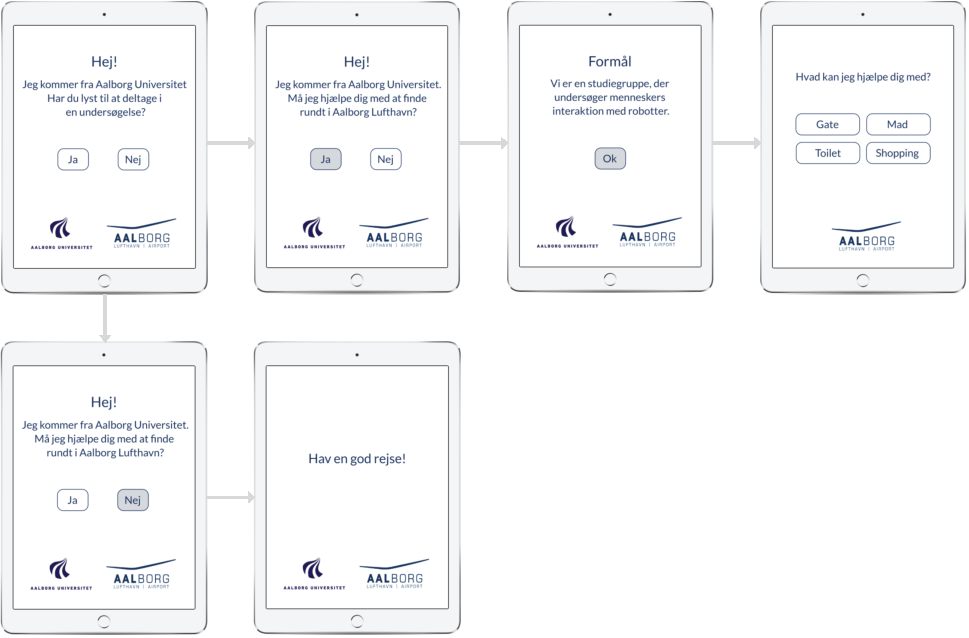
\includegraphics[width = 0.6\textwidth]{Figure/SamledeWirefram} 
\caption{Oversigt over de forskellige skærmbilleder i det samlede \textit{wirefram}.}
\label{fig:SamledeWirefram}
\end{figure}
\noindent
%  

\subsubsection*{Gate information}
%
Testpersonerne får fortalt, at deres opgave er at finde information om deres gate, hvilket skal foregå ved hjælp af robotten. På \autoref{fig:GateInformation} fremgår de forskellige skærmbilleder relevant for dette brugsscenarie. 
%
\begin{figure}[H]
\centering

\includegraphics[width = 0.6\textwidth]{Figure/GateInformation} 
\caption{Oversigt over de forskellige skærmbilleder, der anvendes i brugsscenariet: Gate information.}
\label{fig:GateInformation}
\end{figure}
\noindent
%  

\subsubsection*{Toiletfaciliteter}
%
Testpersonerne får fortalt, at deres opgave er at finde toiletfaciliteter, hvilket skal foregå ved hjælp af robotten. På \autoref{fig:Toiletfaciliteter} fremgår de forskellige skærmbilleder relevant for dette brugsscenarie. 
%
\begin{figure}[H]
\centering

\includegraphics[width = 0.7\textwidth]{Figure/Toiletfaciliteter} 
\caption{Oversigt over de forskellige skærmbilleder, der er specifikke for brugsscenariet: Toiletfaciliteter.}
\label{fig:Toiletfaciliteter}
\end{figure}
\noindent
%  
\subsubsection*{Indkøbsmuligheder}
Testpersonerne får fortalt, at deres opgave er at finde indkøbsmuligheder, hvilket skal foregå ved hjælp af robotten. På \autoref{fig:Indkoebsmuligheder} fremgår de forskellige skærmbilleder relevant for dette brugsscenarie. 
%
\begin{figure}[H]
\centering
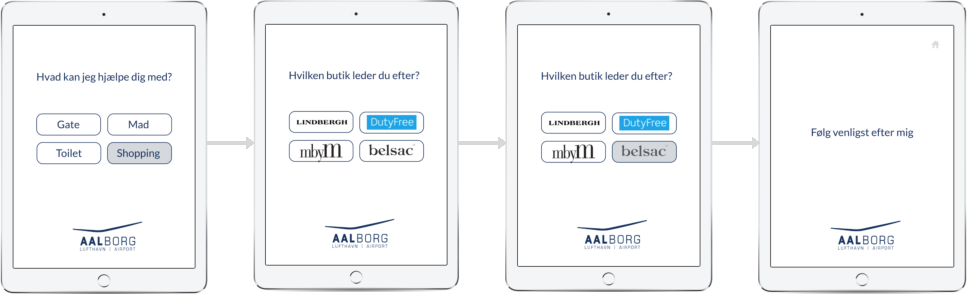
\includegraphics[width = 0.6\textwidth]{Figure/Indkoebsmuligheder} 
\caption{Oversigt over de forskellige skærmbilleder, der anvendes i brugsscenariet: Indkoebsmuligheder.}
\label{fig:Indkoebsmuligheder}
\end{figure}
\noindent
% 
